\documentclass[10pt,letterpaper]{article}
\usepackage[margin=0.78in,headheight=14pt]{geometry}
\usepackage[T1]{fontenc}
\usepackage{lmodern,amsmath,amssymb,booktabs,array,tabularx,microtype}
\usepackage{tikz}
\usetikzlibrary{arrows.meta,positioning,calc}
\usepackage{xcolor,enumitem,fancyhdr,hyperref}
\definecolor{ink}{HTML}{18354A}
\definecolor{accent}{HTML}{176B79}
\hypersetup{colorlinks=true,linkcolor=accent,citecolor=accent,urlcolor=accent,pdftitle={SpatialReadout: multiscale delta-rule memory and a final spatial ConvGRU},pdfauthor={Visual Attention and Working Memory project}}
\pagestyle{fancy}\fancyhf{}\fancyhead[L]{\small SpatialReadout: architecture and decision logic}\fancyhead[R]{\small Source-audited technical paper}\fancyfoot[C]{\thepage}
\setlength{\parindent}{0pt}\setlength{\parskip}{5pt}
\renewcommand{\tabularxcolumn}[1]{>{\raggedright\arraybackslash}p{#1}}
\setlist{nosep,leftmargin=*}
\newcommand{\R}{\mathbb{R}}
\newcommand{\cat}{\mathbin\Vert}
\newcommand{\src}[1]{\textcolor{accent}{\textsf{[#1]}}}
\newcommand{\takeaway}[1]{\par\smallskip\noindent\textbf{Takeaway.} #1}
\newcommand{\psection}[1]{\clearpage\section{#1}}
\begin{document}
\thispagestyle{empty}
{\color{ink}\LARGE\bfseries SpatialReadout: Multiscale Delta-Rule Memory\\[3pt] and a Final Spatial ConvGRU\par}
\vspace{8pt}
{\large Architecture, computational motivations, and limits of interpretation}\par
\vspace{4pt}
{\small Visual Attention and Working Memory project\quad\textbullet\quad Local source snapshot, 29 September 2026}
\vspace{8pt}
\begin{abstract}
\noindent This paper specifies the current \texttt{SpatialReadout} model, rather than its historical global-GRU predecessor or an isolated KDA module. Centered, three-frame RGB stacks pass through four convolutional blocks. Three spatial Kimi Delta Attention (KDA) accumulators, interleaved at $25\times25$, $13\times13$, and $7\times7$, contribute local associative memory to the feedforward hierarchy. The deepest $160\times7\times7$ field is projected to 64 channels and integrated by a final convolutional gated recurrent unit (ConvGRU). Only its terminal $64\times7\times7$ state is flattened and projected to 256 features for a task-specific linear head. An independent CPU constructor audit gives \textbf{1,383,028 trainable parameters}. We derive the exact decay--correction--read update, its signed temporal coefficients, and the implemented write/reset convention. The principal design decision is to postpone \emph{global} compression until after final recurrence, while retaining spatially organized encoder memory. This supplies an inductive bias, not proof of better retention, comparison learning, or biological equivalence. We distinguish documented design intent from plausible but untested explanations, and separate the current fresh-origin training lineage from an earlier warm-start branch. No training, trained-model inference, or new behavioral experiment was performed for this paper.
\end{abstract}
\section{Scope and scientific question}
Visual working-memory tasks require an observer to encode evidence, retain task-relevant information, and convert that information into a report. These requirements are not interchangeable: a representation may contain a cue without applying its meaning, or retain sensory information without learning the required comparison. An architecture description should therefore explain what computations are available without treating their availability as evidence that training discovered them.

The present observer combines two kinds of recurrence. The encoder carries matrix-valued associative states at three spatial scales; a final ConvGRU carries a feature field at the coarsest scale. The motivating question is whether a spatially structured final recurrent substrate is a more suitable place to integrate the encoder's output than a small vector produced by flattening and projecting \emph{before} recurrence. The implementation makes this substitution without adding a controller, top-down feedback, a hand-designed comparator, a transformer, or spatial softmax attention.\src{S1,S2}

The source authority is the current model and its imported definitions, not the older September KDA report. Historical \texttt{README.md}, \texttt{BRIEF.md}, and journal entries record the original warm-start experiment; the current \texttt{FreshRun} worker constructs every learned tensor anew, and \texttt{ContinuationRun} restores that same fresh-origin model at update 7,739. Retained Python member names support historical migration but do not imply old learned-weight inheritance in the fresh run.\src{S1,S4,S5,S8}

This is an architecture paper, not a report of the paused neuroscience study. Source inspection, algebra, parameter counting, and PDF checks are the evidence presented here. No validation score is treated as current live status, and the authorized continuation target is not represented as completed training.

\psection{End-to-end computation and notation}
\begin{figure}[h!]
\centering
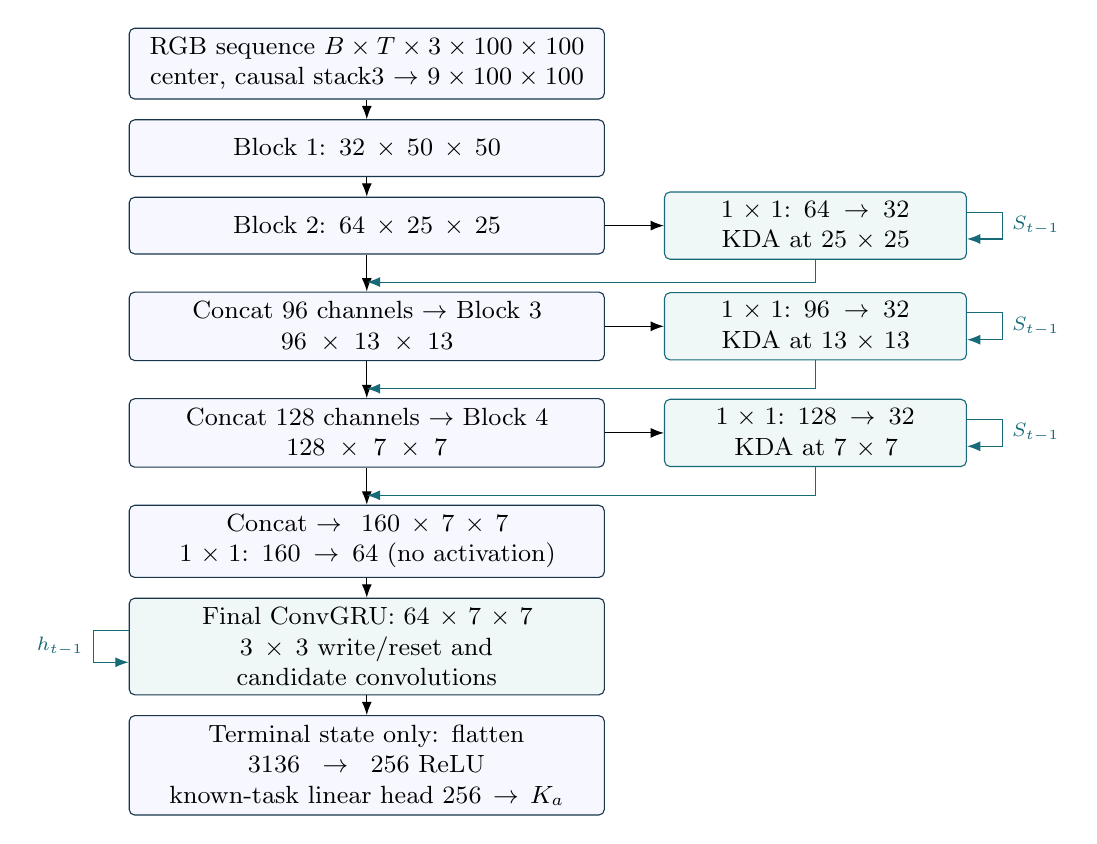
\begin{tikzpicture}[font=\small,>=Latex,box/.style={draw=ink,rounded corners=2pt,fill=blue!3,align=center,minimum height=0.72cm,text width=5.8cm},mem/.style={draw=accent,rounded corners=2pt,fill=teal!6,align=center,text width=3.6cm,minimum height=0.78cm},node distance=0.25cm]
\node[box] (input) {RGB sequence $B\times T\times3\times100\times100$\\center, causal stack3 $\rightarrow9\times100\times100$};
\node[box,below=of input] (b1) {Block 1: $32\times50\times50$};
\node[box,below=of b1] (b2) {Block 2: $64\times25\times25$};
\node[mem,right=0.75cm of b2] (m1) {$1\times1$: $64\to32$\\KDA at $25\times25$};
\node[box,below=0.47cm of b2] (b3) {Concat $96$ channels $\to$ Block 3\\$96\times13\times13$};
\node[mem,right=0.75cm of b3] (m2) {$1\times1$: $96\to32$\\KDA at $13\times13$};
\node[box,below=0.47cm of b3] (b4) {Concat $128$ channels $\to$ Block 4\\$128\times7\times7$};
\node[mem,right=0.75cm of b4] (m3) {$1\times1$: $128\to32$\\KDA at $7\times7$};
\node[box,below=0.47cm of b4] (proj) {Concat $\to160\times7\times7$\\$1\times1$: $160\to64$ (no activation)};
\node[box,below=of proj,fill=teal!6] (gru) {Final ConvGRU: $64\times7\times7$\\$3\times3$ write/reset and candidate convolutions};
\node[box,below=of gru] (head) {Terminal state only: \mbox{flatten} $3136\to256$ ReLU\\known-task linear head $256\to K_a$};
\foreach \a/\b in {input/b1,b1/b2,b2/b3,b3/b4,b4/proj,proj/gru,gru/head}{\draw[->] (\a)--(\b);}
\foreach \a/\b/\c in {b2/m1/b3,b3/m2/b4,b4/m3/proj}{\draw[->] (\a.east)--(\b.west);\draw[->,accent] (\b.south)|- ($(\c.north)+(0,0.12)$);\draw[->,accent] ($(\b.east)+(0,0.17)$) -- ++(0.45,0) -- node[right,font=\scriptsize] {$S_{t-1}$} ++(0,-0.34) -- ($(\b.east)+(0,-0.17)$);}
\draw[->,accent] ($(gru.west)+(0,0.20)$) -- ++(-0.45,0) -- node[left,font=\scriptsize] {$h_{t-1}$} ++(0,-0.40) -- ($(gru.west)+(0,-0.20)$);
\end{tikzpicture}
\caption{One causal time step, repeated for every presented frame. Side branches emit 32 channels and retain separate matrix states; they are not global attention layers. Loops indicate state carried from the preceding update. The last readout is applied only after the final step. Batch dimensions are omitted within the diagram.}
\end{figure}
\vspace{-5pt}
\begin{tabularx}{\linewidth}{@{}lX@{}}\toprule
Symbol & Meaning and dimensions (one episode unless shown)\\\midrule
$X_t,x_t$ & Raw RGB frame; centered three-frame input, $9\times100\times100$.\\
$H_t^s,U_t^s,O_t^s$ & CNN block field, 32-channel projection, and 32-channel KDA emission.\\
$S_t^{s,p,j}$ & Local memory at scale $s$, site $p$, head $j$: $8\times16$.\\
$q_t,k_t,v_t$ & Query/key vectors in $\R^8$ and value vector in $\R^{16}$, per site/head.\\
$\alpha_t,\beta_t$ & Eight row-decay gates and one write-strength gate per site/head.\\
$z_t,h_t,w_t,r_t$ & Projected field, ConvGRU state, write and reset fields: $64\times7\times7$.\\
$a,K_a$ & Externally supplied task identifier and its number of output classes.\\\bottomrule
\end{tabularx}

\psection{Sensory interface and the multiscale encoder}
\subsection{Causal frame stacking has a specific boundary condition}
The suite supplies float32 images in $[0,1]$, laid out as $B\times T\times3\times100\times100$. Centering subtracts $0.5$; it does not divide by $0.5$. For zero-based $t$, define
\begin{equation}
\bar X_t=\begin{cases}X_t-0.5,&t\geq0,\\0,&t<0,\end{cases}
\qquad x_t=\bar X_{t-2}\cat\bar X_{t-1}\cat\bar X_t .
\end{equation}
Here $\cat$ concatenates channels in oldest-to-current order. Padding is created \emph{after} centering, so missing history is zero in centered coordinates (equivalent to raw midgray), not centered black. The first input is $[0,0,X_0-0.5]$ and the second is $[0,X_0-0.5,X_1-0.5]$. No future image enters an earlier update.\src{S2,S6}

Stacking supplies a short explicit temporal window, useful in principle for local changes and motion without requiring recurrence to reconstruct every adjacent-frame difference. This is a computational rationale, not a measured contribution here. It also changes the interpretation of a delay: the first two nominal blank updates can still expose earlier stimulus images. Clean recurrent retention must be distinguished from access through this window.

\subsection{Four blocks, three interleaved memories}
Each block is a biased convolution followed by GroupNorm with eight groups and ReLU. The verified GroupNorm epsilon is $10^{-5}$ and the normalization has learned per-channel scale and shift. The first convolution has kernel 5, stride 2, padding 2; all remaining block convolutions use kernel 3, stride 2, padding 1. There is no pooling.\src{S2}\par
\begin{table}[h!]
\centering\small
\begin{tabular}{@{}lllr@{}}\toprule
Stage & Input channels & Output field & Parameters\\\midrule
Block 1: Conv5/GN/ReLU & 9 & $32\times50\times50$ & 7,296\\
Block 2: Conv3/GN/ReLU & 32 & $64\times25\times25$ & 18,624\\
Projection 1; KDA 1 & $64\to32$ & $32\times25\times25$ & $2,080+24,754$\\
Block 3: Conv3/GN/ReLU & $64+32=96$ & $96\times13\times13$ & 83,232\\
Projection 2; KDA 2 & $96\to32$ & $32\times13\times13$ & $3,104+24,754$\\
Block 4: Conv3/GN/ReLU & $96+32=128$ & $128\times7\times7$ & 147,840\\
Projection 3; KDA 3 & $128\to32$ & $32\times7\times7$ & $4,128+24,754$\\\bottomrule
\end{tabular}
\caption{Constructor-verified counts; output sizes are analytically propagated from the actual convolution attributes. Each projection is a biased $1\times1$ convolution. No trained forward pass was needed.}
\end{table}
For each memory-bearing scale, $U_t^s=P_sH_t^s$ drives a KDA update and the next block receives $H_t^s\cat O_t^s$. Consequently the next scale sees both contemporary CNN features and a learned memory emission, not only a memory-compressed replacement. At the deepest scale the same concatenation gives $160\times7\times7$. The three modules have distinct weights and states; they are neither weight-tied nor three successive global token-mixing layers.

GroupNorm avoids batch-dependent normalization statistics, consistent with the small physical microbatch used in training \cite{gn}. It does, however, aggregate within channel groups \emph{over spatial positions}. Therefore ``local KDA state'' does not mean the entire encoder is strictly spatially isolated: convolutional neighborhoods, GroupNorm statistics, and subsequent layers couple information across the field.
\takeaway{Spatial organization survives the encoder, but resolution and channels are already compressed. ``Compression after recurrence'' means postponing the large global flatten/projection, not eliminating every bottleneck.}

\psection{Exact spatial KDA: decay, corrective write, and read}
\subsection{What is parameterized at each scale}
The 32-channel projected field passes through a biased $3\times3$ convolution with padding 1, producing 82 channels. These are reshaped to $B\times H\times W\times2\times41$. For each head, the packed components are $q_8,k_8,v_{16},\alpha_8,\beta_1$. Queries and keys are normalized by
\begin{equation}
\mathcal N(u)=u/\max(\lVert u\rVert_2,10^{-6}),\qquad
q_t=\mathcal N(\tilde q_t),\quad k_t=\mathcal N(\tilde k_t).
\end{equation}
The value is unconstrained; $\alpha_t=\sigma(\tilde\alpha_t)$ and $\beta_t=\sigma(\tilde\beta_t)$. Thus $\alpha_t$ and $\beta_t$ are nonnegative sigmoid gates, \emph{not} the signed coefficients discussed below. Each head stores $S_t\in\R^{8\times16}$; the complete tensor is $B\times H\times W\times2\times8\times16$. All three scales begin with zero state in every call to the sequence model.\src{S1--S3}

Suppress scale, site, head, and episode indices. With column vectors and $D_t=\operatorname{diag}(\alpha_t)$, the implementation is exactly
\begin{align}
\bar S_t &= D_t S_{t-1}, &&\text{decay each key row},\label{eq:decay}\\
e_t &= v_t-\bar S_t^{\mathsf T}k_t, &&\text{current-key prediction error},\\
S_t &= \bar S_t+\beta_t k_t e_t^{\mathsf T}, &&\text{rank-one corrective write},\label{eq:write}\\
o_t &= S_t^{\mathsf T}q_t, &&\text{read the updated state}.\label{eq:read}
\end{align}
The two 16-dimensional reads are concatenated into 32 channels and passed through a biased $1\times1$ convolution, producing $O_t^s$. There is no softmax, output normalization, or extra nonlinearity within this emission. The $3\times3$ packed-input convolution has 23,698 parameters, and the output convolution has 1,056: 24,754 per KDA module.\src{S3}

\subsection{Connection to Kimi Delta Attention, without importing another model}
Expanding the error in Eq.~\eqref{eq:write} gives
\begin{equation}
S_t=A_tS_{t-1}+\beta_t k_tv_t^{\mathsf T},\qquad
A_t=(I-\beta_t k_tk_t^{\mathsf T})D_t.\label{eq:transition}
\end{equation}
This is the diagonal-gated delta-rule recurrence of Kimi Linear, Eq.~1 \cite{kda}. The ordering matters: decay precedes error correction, and the read uses the \emph{updated} state. In general $D_t$ and $k_tk_t^{\mathsf T}$ do not commute. Describing a scalar-decay DeltaNet or moving decay after the correction would not specify this implementation.

The relationship is mathematical, not architectural identity. This observer does not instantiate Kimi Linear's language model, hybrid full-attention layers, mixture of experts, or chunkwise accelerator kernel. It uses a small, explicit, per-location spatial adaptation with two heads and sequential updates. The word ``attention'' in its name is not evidence for patch-to-patch competition.

Initialization makes the nine gate outputs per head input-independent: gate convolution weights are zero, the eight decay biases are $\log9$, and the write bias is zero. Hence initially $\alpha=0.9$ and $\beta=0.5$ everywhere. These parameters remain trainable; a fixed initial retention is not a fixed lifetime throughout learning. Other packed channels use ordinary constructor initialization.
\takeaway{The memory stores local channel associations, writes the discrepancy from its current prediction, and reads after that correction.}

\psection{What KDA remembers---and what its coefficients mean}
\subsection{Error correction rather than indiscriminate accumulation}
For a unit-norm key, the prediction at the just-written key satisfies
\begin{equation}
S_t^{\mathsf T}k_t=(1-\beta_t)\bar S_t^{\mathsf T}k_t+\beta_tv_t .\label{eq:interpolation}
\end{equation}
This follows directly from Eq.~\eqref{eq:write}, not from a behavioral experiment. It explains the attraction of a delta rule: repeated evidence for the same key corrects a prediction rather than simply adding the full value repeatedly. The identity assumes a unit key; the epsilon safeguard can yield a smaller norm for nearly zero packed vectors. For a general key, the effective correction along that key includes $\lVert k_t\rVert^2$.

The channelwise gate allows the eight key rows of one head to retain different fractions of their previous contents. It does not select a spatial location by normalizing against other locations. A gate map can vary spatially because it is generated from spatial features, while the state update remains an $8\times16$ operation at each site. Two heads provide two independently parameterized association/read paths before their emissions are mixed. Whether two heads, eight keys, or sixteen values are optimal is not established by this audit.

\subsection{Signed temporal coefficients}
For zero initial state, unrolling Eq.~\eqref{eq:transition} yields
\begin{align}
S_t&=\sum_{\tau=0}^{t}P_{t,\tau}\,\beta_\tau k_\tau v_\tau^{\mathsf T},\\
P_{t,\tau}&=A_tA_{t-1}\cdots A_{\tau+1},\qquad P_{t,t}=I,\\
o_t&=\sum_{\tau=0}^{t}c_{t,\tau}v_\tau,\qquad
c_{t,\tau}=\beta_\tau q_t^{\mathsf T}P_{t,\tau}k_\tau.\label{eq:coeff}
\end{align}
Queries, keys, and transition products can generate either sign for $c_{t,\tau}$. These coefficients need not sum to one. They express how earlier \emph{values at one head/site} contribute to the current pre-output read along the observed computation, not a probability distribution over source patches. The output convolution subsequently mixes the heads and channels; deeper processing and the final task head further transform the result.

The expansion is an exact conditional decomposition given the realized gates, queries, keys, and values. It is not a claim that changing an input value while holding all other quantities fixed reproduces a full counterfactual trial. In particular, later-scale inputs depend on earlier recurrent emissions. A coefficient is neither an input-independent causal influence nor automatic attribution of the final choice.

\subsection{State footprint and spatial interpretation}
At each scale there are $2\cdot8\cdot16=256$ stored scalars per spatial site. The three memories hold 160,000, 43,264, and 12,544 scalars per episode, respectively. These are activation-state sizes, not trainable parameter counts. They remain fixed as sequence length grows, but the unrolled training graph need not have constant memory cost. The Python sequence loop carries differentiable state across the full episode.

Convolutions allow neighboring inputs to influence the packed local variables; multiscale concatenation allows lower-scale memory emissions to affect deeper memories. GroupNorm further couples spatial statistics. Thus it is accurate to call the recurrence \emph{site-indexed}, but inaccurate to portray an individual cell as an isolated image pixel or a spatially segregated biological neuron.
\takeaway{Learned retention gates are positive; implicit read coefficients can be signed. Neither is a global spatial softmax.}

\psection{Final spatial recurrence and terminal compression}
\subsection{The exact ConvGRU convention}
Let $F_t=H_t^3\cat O_t^3\in\R^{160\times7\times7}$ denote the deepest concatenation (the three memory-bearing scales are indexed $s=1,2,3$). A biased $1\times1$ projection gives $z_t\in\R^{64\times7\times7}$, with no activation or extra normalization. With $h_{-1}=0$, the final recurrent cell is
\begin{align}
[w_t,r_t]&=\sigma\!\left(W_g* [z_t\cat h_{t-1}]+b_g\right),\label{eq:gates}\\
\tilde h_t&=\tanh\!\left(W_c*[z_t\cat(r_t\odot h_{t-1})]+b_c\right),\\
h_t&=(1-w_t)\odot h_{t-1}+w_t\odot\tilde h_t.\label{eq:convgru}
\end{align}
The first 64 channels of the gate output are \emph{write}, and the next 64 are reset. A large $w_t$ replaces old state with the candidate; it is not the retention coefficient. Reset is applied to the old hidden field \emph{before} the candidate convolution. Both convolutions have kernel 3, padding 1, stride 1. The gate convolution maps $128\to128$ channels; the candidate maps $128\to64$.\src{S1}

Gated recurrent units provide learned retention and update paths \cite{gru}; convolutional variants replace dense spatial connectivity with spatially shared kernels \cite{convgru}. Those precedents motivate the operation, but the local source is the authority for this particular reset placement and write convention. There is no separate state-to-encoder feedback connection. The final hidden field influences its own next update, not the upstream CNN or KDA modules.

Both recurrent biases are explicitly zero. Conv/Linear weights use the ordinary PyTorch reset convention documented in the model (Kaiming-uniform with $a=\sqrt5$); projection and readout biases retain their default fan-in-uniform initialization. Zero gate bias alone does \emph{not} mean all initial gates equal $0.5$, since their weights and inputs are nonzero. This differs from the explicit zero gate weights used in KDA.

\subsection{Compression occurs after the final recurrent update}
After all $T$ updates, the sole reported output is
\begin{equation}
f=\operatorname{ReLU}(W_f\operatorname{vec}(h_{T-1})+b_f),\qquad
\ell_a=W_af+b_a,\quad f\in\R^{256}.\label{eq:head}
\end{equation}
There is no temporal average, pooled spatial mean, intermediate classification loss, dropout, final LayerNorm, or final global GRU. Flattening retains coordinate-specific inputs to a dense map, rather than making the decision translation-invariant. Only the linear head selected by the supplied task name is executed.
\begin{table}[h!]
\centering\small
\begin{tabular}{@{}llr@{}}\toprule
Module & Weight operation & Parameters\\\midrule
Spatial input & Conv1, $160\to64$ & 10,304\\
Gate convolution & Conv3, $128\to128$ & 147,584\\
Candidate convolution & Conv3, $128\to64$ & 73,792\\
Terminal readout & Linear, $3136\to256$ & 803,072\\
All 13 task heads & Linear, $256\to K_a$ & 7,710\\\midrule
All CNN blocks / KDA projections / KDA & & $256,992/9,312/74,262$\\
\textbf{Complete model} & \textbf{All trainable} & \textbf{1,383,028}\\\bottomrule
\end{tabular}
\caption{All biases and normalization affine parameters are included. The ConvGRU has 221,376 parameters and a 3,136-scalar hidden state per episode.}
\end{table}

\psection{Task interface and current training lineage}
\begin{table}[h!]
\centering\small
\begin{tabularx}{\linewidth}{@{}lclX@{}}\toprule
Task identifier & $K_a$ & Head params & Label meaning\\\midrule
\texttt{motion\_direction} &4&1,028& Right, up, left, down\\
\texttt{orientation} &2&514& Negative / positive axial change\\
\texttt{contrast} &2&514& Frame 0 / frame 1\\
\texttt{spatial\_frequency} &2&514& Frame 0 / frame 1\\
\texttt{chromatic\_increment} &2&514& Frame 0 / frame 1\\
\texttt{contour} &2&514& Frame 0 / frame 1\\
\texttt{natural\_spectrum} &2&514& Frame 0 / frame 1\\
\texttt{orientation\_ring} &2&514& Negative / positive axial change\\
\texttt{orientation\_cued} &2&514& Unchanged/opposite cue sign / in cue sign\\
\texttt{motion\_duration\_cued} &4&1,028& Right, up, left, down\\
\texttt{krauzlis\_cued\_motion} &2&514& Foil-only or catch / target change\\
\texttt{spatial\_binding} &2&514& Foil-only exchange / target exchange\\
\texttt{image\_recognition} &2&514& Not in study set / in study set\\\bottomrule
\end{tabularx}
\caption{Exact catalog identifiers and class counts. Binary heads do not all mean ``change versus no change.'' The 13 tasks comprise 35 catalog conditions.\src{S6}}
\end{table}
The task identifier routes the terminal features to an output head; it is not a learned task inference system and is not supplied as a feature to the encoder. Images are the shared trunk's input. The training loop discards batch metadata before calling the model. Task-known routing must not be confused with knowing the target location, cue sign, or correct answer within an episode.\src{S1,S7}

\textbf{Acquisition recipe.} All learned parameters are trainable in float32. One Adam optimizer \cite{adam} uses learning rate $10^{-4}$, $\beta_1=0.9$, $\beta_2=0.999$, $\epsilon=10^{-8}$, and zero weight decay. An effective batch of 32 is accumulated from eight microbatches of four from the scheduled task/condition. Each microbatch mean cross-entropy is multiplied by $4/32$ before backpropagation. The optimizer steps once after accumulation and finite-gradient checks; gradients are never clipped. TF32 is disabled in the run configuration.\src{S4,S7}

There is no temporal detach in the model. Each complete episode is unrolled and its final loss backpropagates through the final ConvGRU and all three encoder memories. States reset at every sequence call, so microbatch accumulation combines parameter gradients, not memory across episodes. All heads are trainable in principle, but only the selected head obtains gradients on a particular update. Task and condition queues provide balanced scheduling without altering native sequence lengths.\src{S1,S2,S7}

\textbf{Fresh origin, unchanged continuation.} The fresh worker seeds construction with 98192763 and begins with no checkpoint input, optimizer history, stream history, or inherited learned weights. Disposable profiling state is not production initialization. The authorized continuation resumes the fresh-run terminal at cumulative update \textbf{7,739}, preserving model, Adam, scheduler, streams, and RNG, with a target of \textbf{104,000 additional updates}, or \textbf{111,739 cumulative}. These are the declared starting point and horizon, not a claim of completion or current live progress.\src{S4,S5}

Continuation selection remains validation-only: equal-task mean AUC, then equal-task chance-normalized balanced accuracy, retaining earlier ties. Ten planned looks occur every 10,400 additional updates. A later optimizer step cannot inherit an earlier checkpoint's measured score. No live status was fetched for this paper.

\psection{Design decisions: intended problem and evidential limit}
\subsection{Why move recurrence ahead of global compression?}
The historical encoder emitted the same $160\times7\times7$ field, flattened it at \emph{every} time step, projected it to 256 with ReLU, and passed those vectors to a 256-dimensional global GRU. The current subclass deletes \texttt{feat}, \texttt{gru}, and \texttt{norm}; it does not secretly execute them before the spatial cell.\src{S1,S2}

The change places a 3,136-scalar, coordinate-indexed state between the encoder and the final 256-feature bottleneck. In the older ordering, the final recurrent module had access only to the already-compressed vector. In the new ordering, neighboring locations can interact through recurrent convolutions before the terminal global map. The documented intent is to preserve spatial structure through final recurrence, keep all three KDA modules, and change only that readout pathway.\src{S8}

This is not a theorem that the historical projection destroyed relevant information. A learned 256-dimensional code may suffice for a task; a larger spatial state may still fail to learn its rule. The new $160\to64$ projection remains a channel bottleneck, the CNN still downsamples, and the final $3136\to256$ map can discard information. What changes is the \emph{location and structure} of compression, not its absence.

\subsection{A decision ledger}
\begin{table}[h!]
\small
\begin{tabularx}{\linewidth}{@{}>{\raggedright\arraybackslash}p{0.23\linewidth}XX@{}}\toprule
Choice & Computational purpose & What is not established\\\midrule
Retain three KDA scales & Preserve recurrent encoder pathways at different resolutions; explicit scope in brief. & That all scales are necessary or optimally placed.\\
Keep current plus emitted fields & Let the next block use present features alongside memory-derived features. & That learned weights exploit both pathways.\\
$160\to64$ pointwise projection & Match the final recurrent channel width without collapsing coordinates. & Optimal width or information preservation.\\
$3\times3$ final ConvGRU & Share local spatial update kernels while maintaining a field-valued state. & Superiority to dense, larger-kernel, or other recurrent cells.\\
Terminal flatten, not pooling & Permit coordinate-specific decisions after temporal integration. & Translation robustness or abstraction from fixed layout.\\
No new controller/comparator & Keep the architectural change bounded and leave task-rule acquisition to training. & That task-conditioned comparisons emerge automatically.\\
Task-specific heads & Respect different output vocabularies with a shared trunk. & Task inference or interference-free joint learning.\\\bottomrule
\end{tabularx}
\caption{The retained/replaced modules are documented decisions. Mechanistic purposes in the middle column are computational interpretations unless explicitly described as scope; the right column prevents those interpretations becoming causal claims.}
\end{table}
\subsection{Why the two recurrent mechanisms are not redundant by definition}
KDA maintains local key--value association matrices and can selectively correct a prediction in a learned key direction. The final ConvGRU maintains a feature field and combines a candidate with its previous state through channel/site-wise gates. Its convolutions also operate over the previous spatial hidden field. These are different update families and occupy different levels of the hierarchy. They may complement one another, duplicate useful functions, or interfere during joint learning. Only controlled removal/replacement and matched training would discriminate those possibilities.

\psection{Interpretation, limitations, and discriminating tests}
\subsection{An approximate computational observer, not a primate circuit}
The architecture supplies explicit state, learned forgetting, and spatially organized recurrent computation. These are useful abstractions for asking how an observer can use temporally separated visual evidence. They do not identify anatomical areas, neuronal types, synaptic time constants, or a physiological stimulation substrate. Signed feature channels and $8\times16$ matrix entries should not be called firing rates or biological synapses without an additional measurement model.

It is useful to distinguish learned weights, which persist across episodes, from recurrent states, which reset. Calling the former ``long-term memory'' and the latter ``working memory'' is at most a modeling analogy. The architecture does not implement a separate biological consolidation process. Similarly, learned gates can support selective retention but are not, by themselves, evidence for attentional allocation. The repository analysis SOP requires behavioral cueing and controlled interventions to support such claims.\src{S9}

\subsection{What the architecture audit can and cannot establish}
This paper establishes the source-defined computation and constructor counts. It does not establish task competence, improved sensitivity, an optimal memory lifetime, convergence, or superiority to the old model. Historical warm-start experiments carried trained CNN/KDA/head tensors while introducing new spatial recurrence/readout tensors. Unequal experience and an unmatched control prevent attributing their outcomes solely to the architectural replacement. The current fresh-origin lineage removes that particular inheritance at initialization, but one lineage alone still does not provide a matched causal architecture comparison.\src{S4,S8}

A label decoder that extracts information from a frozen representation is not proof that the deployed head uses it. Likewise, externally retaining sample-time activations gives an analysis readout access that the deployed terminal-only head does not have. These distinctions are especially important when interpreting relational tasks: accessible cue and orientation features do not guarantee a learned cue-conditioned comparison. No explicit comparison operator is present here.

\subsection{Tests that would resolve specific design uncertainties}
\begin{enumerate}[label=\textbf{\arabic*.}]
\item \textbf{Compression order.} Compare fresh global-GRU and spatial-ConvGRU models under matched tasks, exposure, selection, and multiple seeds. Account separately for parameter budget and recurrent-state size; merely training both for the same wall time changes exposure.
\item \textbf{Memory necessity.} Remove or reset individual KDA states or the final ConvGRU at declared epochs, with matched trials and sham controls. A global reset is not a spatial inhibition experiment; perturbing an emitted field is not erasing the module's stored matrix.
\item \textbf{Retention versus stacked sensory access.} Test genuinely stimulus-free updates after the explicit frame window has cleared. Preserve the nonblank raster evidence when comparing delays; nominal delay labels alone are insufficient.
\item \textbf{Rule acquisition versus accessibility.} Compare capacity-matched terminal-only readouts and temporal-access diagnostics under declared supervision. Do not interpret auxiliary-supervised success as native-label learning by the deployed model.
\item \textbf{Selection and spatial effects.} Measure paired psychometric changes for relevant and irrelevant evidence, separating sensitivity from response bias. Known task routing does not supply a valid/invalid cue manipulation, and a fixed-terminal classifier has no reaction-time policy.
\end{enumerate}
These are proposed discriminating experiments, not additional work executed for this paper. They preserve the distinction between a reasonable design rationale, a correlational diagnostic, and a causal architectural result.
\takeaway{The model makes spatial temporal integration available; whether training uses it for the intended evidence-selection and comparison rules remains an empirical question.}

\psection{Reproducibility and source map}
\small
The editable source, constructor audit, complete SHA-256 manifest, and PDF verification receipts are colocated in this repository directory:
\begin{center}\path{SecondPass/SpatialReadout/ArchitecturePaper/}\end{center}
Counts were obtained with PyTorch 2.8.0 on CPU with intra/inter-op threads limited to two. No checkpoint was loaded; no model forward/backward, dataset download, optimizer update, or accelerator operation was used. Shapes in Tables 1--2 follow the actual constructor attributes and convolution output formula. Biases and GroupNorm affine tensors are included; temporary inherited modules deleted by the subclass are excluded.

\begin{tabularx}{\linewidth}{@{}lX@{}}\toprule
Code & Repository-relative authority and relevant content\\\midrule
S1 & \path{SecondPass/SpatialReadout/model.py}, lines 13--51: final cell, subclass, sequence reset, terminal head.\\
S2 & \path{WorkingMemory/PlainBaseline/accum.py}, lines 40--75: blocks, projections, stacking, encoder; old vector readout.\\
S3 & \path{PreAttentiveVision/TemporalIntegration/accumulators.py}, lines 19--66: KDA update, packing, initialization, states.\\
S4 & \path{SecondPass/SpatialReadout/FreshRun/worker.py}: fresh constructor/provenance, Adam, precision, namespaces.\\
S5 & \path{SecondPass/SpatialReadout/ContinuationRun/worker.py} and \path{README.md} in that directory: exact restore, source7739, authorized horizon.\\
S6 & \path{SecondPass/TaskSuite/catalog.json} and \path{suite.py}: input contract, conditions, labels, head sizes.\\
S7 & \path{SecondPass/JointTraining/worker.py}, update lines 51--90; \path{core.py} scheduler; \path{SecondPass/SpatialComparisonReadout/CloudRun/worker.py}, line65: reused update adapter, not a different model.\\
S8 & \path{SecondPass/SpatialReadout/BRIEF.md}, \path{README.md}; \path{LabJournal/spatial-readout-convgru.md}: historical intent and warm-start caveats.\\
S9 & \path{ANALYSIS_SOP.md}: computational-observer interpretation and analysis safeguards.\\\bottomrule
\end{tabularx}

\textbf{Identity and scope.} The worktree was dirty at audit time, so a commit alone cannot identify the model. The full hash of S1 is given below; \texttt{source\_manifest.json} contains complete hashes of all 15 inspected authority files, and \path{count_verification.json} records every named tensor and count. This binds the paper to local files; it is not a claim that advancing cloud deployment files were independently rechecked.
\begin{center}\footnotesize\texttt{4f88ba0a0cf6abede416f1260a71bc13bfab5cfa51eb00d17e11369301f4d503}\end{center}
\textbf{Build.} Run \texttt{python3 build.py} here (Tectonic is configurable via \texttt{TECTONIC}). Run the CPU interpreter on \texttt{verify\_counts.py} to refresh counts; run \texttt{python3 verify\_pdf.py} for text, bounds, font, page, and rendering checks. The original model/training sources are not modified. The PDF receipt distinguishes automated checks from visual inspection. The local source snapshot, rather than an asserted latest checkpoint score, defines the report's freshness.

\vspace{-7pt}
\begin{thebibliography}{9}\setlength{\itemsep}{1pt}
\bibitem{kda} Kimi Team. \emph{Kimi Linear: An Expressive, Efficient Attention Architecture}. 2025. arXiv:2510.26692v2, Eq.~1. \url{https://arxiv.org/html/2510.26692v2}.
\bibitem{gru} K. Cho, B. van Merrienboer, C. Gulcehre, D. Bahdanau, F. Bougares, H. Schwenk, and Y. Bengio. \emph{Learning Phrase Representations using RNN Encoder-Decoder for Statistical Machine Translation}. EMNLP, 2014. \url{https://arxiv.org/abs/1406.1078}.
\bibitem{convgru} N. Ballas, L. Yao, C. Pal, and A. Courville. \emph{Delving Deeper into Convolutional Networks for Learning Video Representations}. ICLR, 2016. \url{https://arxiv.org/abs/1511.06432}.
\bibitem{gn} Y. Wu and K. He. \emph{Group Normalization}. 2018. \url{https://arxiv.org/abs/1803.08494}.
\bibitem{adam} D. P. Kingma and J. Ba. \emph{Adam: A Method for Stochastic Optimization}. ICLR, 2015. \url{https://arxiv.org/abs/1412.6980}.
\end{thebibliography}
\end{document}
